\documentclass{article}

\usepackage{fancyhdr}
\usepackage{extramarks}
\usepackage{amsmath,siunitx}
\usepackage{amsthm}
\usepackage{amsfonts}
\usepackage{wrapfig}
\usepackage{tikz}
\usepackage[plain]{algorithm}
\usepackage{algpseudocode}
\usepackage{xcolor}
\usetikzlibrary{automata,positioning}

%
% Basic Document Settings
% Template from https://github.com/jdavis/latex-homework-template/blob/master/homework.tex
%

\topmargin=-0.45in
\evensidemargin=0in
\oddsidemargin=0in
\textwidth=6.5in
\textheight=9.0in
\headsep=0.25in

\linespread{1.1}

\pagestyle{fancy}
\lhead{\hmwkAuthorName}
\chead{\hmwkClass\ (\hmwkClassInstructor\ \hmwkClassTime): \hmwkTitle}
\rhead{\firstxmark}
\lfoot{\lastxmark}
\cfoot{\thepage}

\renewcommand\headrulewidth{0.4pt}
\renewcommand\footrulewidth{0.4pt}

\setlength\parindent{0pt}

\newcommand{\enterProblemHeader}[1]{
    \nobreak\extramarks{}{Problem \arabic{#1} continued on next page\ldots}\nobreak{}
    \nobreak\extramarks{Problem \arabic{#1} (continued)}{Problem \arabic{#1} continued on next page\ldots}\nobreak{}
}

\newcommand{\exitProblemHeader}[1]{
    \nobreak\extramarks{Problem \arabic{#1} (continued)}{Problem \arabic{#1} continued on next page\ldots}\nobreak{}
    \stepcounter{#1}
    \nobreak\extramarks{Problem \arabic{#1}}{}\nobreak{}
}

\setcounter{secnumdepth}{0}
\newcounter{partCounter}
\newcounter{homeworkProblemCounter}
\setcounter{homeworkProblemCounter}{1}
\nobreak\extramarks{Problem \arabic{homeworkProblemCounter}}{}\nobreak{}

\newenvironment{homeworkProblem}[1][-1]{
    \ifnum#1>0
        \setcounter{homeworkProblemCounter}{#1}
    \fi
    \section{Problem \arabic{homeworkProblemCounter}}
    \setcounter{partCounter}{1}
    \enterProblemHeader{homeworkProblemCounter}
}{
    \exitProblemHeader{homeworkProblemCounter}
}
%   - Title
%   - Due date
%   - Class
%   - Section/Time
%   - Instructor
%   - Author
%

\newcommand{\hmwkTitle}{Qual Problems}
\newcommand{\hmwkDueDate}{December 19, 2018}
\newcommand{\hmwkClass}{Cosmology}
\newcommand{\hmwkClassTime}{}
\newcommand{\hmwkClassInstructor}{Professor Renee Hlozek}
\newcommand{\hmwkAuthorName}{\textbf{Bethany Ludwig}}

%
% Title Page
%

\title{
    \vspace{2in}
    \textmd{\textbf{\hmwkClass:\ \hmwkTitle}}\\
    \normalsize\vspace{0.1in}\small{Due\ on\ \hmwkDueDate\ at 2:30pm}\\
    \vspace{0.1in}\large{\textit{\hmwkClassInstructor\ \hmwkClassTime}}
    \vspace{3in}
}

\author{\hmwkAuthorName}
\date{}

\renewcommand{\part}[1]{\textbf{\large Part \Alph{partCounter}}\stepcounter{partCounter}\\}

%
% Various Helper Commands
%

% Useful for algorithms
\newcommand{\alg}[1]{\textsc{\bfseries \footnotesize #1}}

% For derivatives
\newcommand{\deriv}[1]{\frac{\mathrm{d}}{\mathrm{d}x} (#1)}

% For partial derivatives
\newcommand{\pderiv}[2]{\frac{\partial}{\partial #1} (#2)}

% Integral dx
\newcommand{\dx}{\mathrm{d}x}

% Alias for the Solution section header
\newcommand{\solution}{\textbf{\large Solution}}

% Probability commands: Expectation, Variance, Covariance, Bias
\newcommand{\E}{\mathrm{E}}
\newcommand{\Var}{\mathrm{Var}}
\newcommand{\Cov}{\mathrm{Cov}}
\newcommand{\Bias}{\mathrm{Bias}}

\begin{document}

\maketitle

\pagebreak

\begin{homeworkProblem}
    {\color{purple}What is recombination? At what temperature did it occur? Explain why this does not match the ionization potential of hydrogen.}\\
    \\ Relevant Equations:
    \begin{enumerate}
        \item \(E = k_bT\) 
        \item \(\frac{n_pn_e}{n_e}\propto T^{3/2}e^{-1/T}\) Saha Equation
        \item \(x_e=\frac{n_e}{n_p+n_H}\) Free Electron Fraction
    \end{enumerate}
    \\
    \solution \\
    \textbf{What is recombination?}\\
    The epoch where a sea of electrons, atomic nuclei, and photons $\rightarrow$ neutral atoms, for the first time.\\
    Temperature dropped due to expansion.\\
    Photoionization no longer occured often enough to maintain the ionization fraction of Hydrogen.\\
    \textbf{At what temperature did it occur?}\\
    Assuming that the reaction happens fast enough to keep things in thermal equilibrium we can use the Saha equation to relate the ionization fraction to the temperature. \\
    \[\frac{n_pn_e}{n_e}\propto T^{3/2}e^{-1/T}\]\\
    This can be further simplified if we require that $n_e=n_p$ and we use the free electron fraction. \\
    The temperature ends up being about $\sim 1/4$ eV or 
    \[\frac{1}{4}\text{eV} \frac{1}{\num{8.6e-5}\text{ eV}} K \approx 3000 \text{ kelvin}\]
    \textbf{Explain why this does not match the ionization potential of hydrogen}\\
    The ionization potential of hydrogen is 13.6 eV or 
    \[13.6\text{eV} \frac{1}{\num{8.6e-5}\text{ eV}} K \approx 150000 \text{ kelvin}\]
    The temperature of recombination is significantly lower than this because CMB photons aren't uniform. The cmb is very close to a blackbody spectrum which has an exponential tail known as the Wien's Tail. This tail contains a non negligible number of photons which are still able to ionize hydrogen. This is made worse by the fact that photons also outnumbered baryons $10^9:1$ because of baryogenesis and the resultant particle/antiparticle annihilation.  
    \\
    \textbf{Follow Up}
    \begin{itemize}
        \item The process was not instantaneous. As recombination progressed, the number of free electrons available for thomson scattering which kpet photons and baryons in thermal equilibrium, decreased. This caused a drop in the opacity for the photons until the optical depth was low enough ($\tau=1$) that photons could stream freely through the universe: The CMB. This corresponds to the surface of last scattering where radiation and matter decoupled.
        \item If the photon:baryon ratio were higher there would be more ionization and recombination would happen later.
        \item If the ionization energy of Hydrogen was lower, it would take longer to cool off significantly past this temperature due to wien's tail so recombination would happen later.
    \end{itemize}
\end{homeworkProblem}
\begin{homeworkProblem}
    {\color{purple}The universe is said to be ``flat", or, close to flat. 
    What are the properties of a flat universe and what evidence do we have for it?}
    \\ Relevant Equations:
    \begin{enumerate}
        \item \( H(t)^2=\frac{8\pi G}{3}\Big[\rho(t)+\frac{\rho_{cr}-\rho_0}{a(t)^2}\Big]\)  Friedman Equation
        \item \(H(a)^2=H_0^2\Big[\Omega_ra^{-4}+\Omega_ma^{-3}+\Omega_ka^{-2}+\Omega_\Lambda\Big]\)Friedman Equation
        \item \(\rho_c = \frac{3 H_0^2}{8\pi G}\) Critical Density
    \end{enumerate}
    \textbf{Solution}\\
     \textbf{What are the properties of a flat universe?}
     \begin{itemize}
         \item Parallel Lines do not Converge or Diverge
         \item Sum of Angles in a triangle = 180 deg
         \item Density of the universe is the critical density
     \end{itemize}
     \textbf{What evidence do we have for it?}\\
     By measuring the density of the universe we can determine the curvature. We can probe the different components many ways (CL Spectrum of CMB, galaxy cluster distribution, etc.). We can also look at the angular scale of CMB fluctuations which depend on the universe's geometry.
    \\
    If the universe were positively curved, the peak of the CMB $C_l$ power spectrum would occur at larger angular scales (lower multipoles) and if it was negatively curved, the peaks would be at smaller angular scales (higher multipoles).
    \\
    Since the expansion rate evolves differently for different densities we can also use Type Ia SNR to map distance to $z$ and infer $\Omega_0$.
    \\ 
    From the Friedman Eq the density of the universe determines its geometry and tells us how the scale factor evolves over time.
    \[\frac{H^2}{H_0^2}=\Omega_r a^{-4}+\Omega_m a^{-3}+\Omega_ka^{-2}+\Omega_\Lambda\]
    \[\Omega_0=\Omega_r+\Omega_m+\Omega_\Lambda,\;\;1-\Omega_0=\Omega_k \rightarrow \text{ if } \Omega_0=1, \Omega_k = 0\]
    \textbf{Follow Up}\\
    The universe was likely much flatter in the early universe as even slight deviations in the density would've changed our expansion significantly. Inflation solves this flatness problem by flattening everything out through exponential expansion, so it doesn't matter how curved the universe was pre inflation.
\end{homeworkProblem}
\pagebreak
\begin{homeworkProblem}
   {\color{purple} Outline the development of the Cold Dark Matter spectrum of density fluctuations from the early universe to the current epoch. \\  
    \\
    Rephrased: Describe how fluctuations in the matter density grow with time in different cosmological epochs and how this leads to the matter power spectrum we see.\\}
    \solution\\
    \textbf{Gravitational instability increases density fluctuations over time.}
    \begin{itemize}
        \item On large scales, the universe is homogenous. 
        \begin{itemize}
            \item But on small scales you see anisotropies with small amplitudes in the cmb that can be described with a gaussian random field.
            \item These become bigger over time.
        \end{itemize}
        \item To talk about this we define a fractional overdensity, or relative density contrast:
        \[\delta=\frac{p(\Vec{r},t)}{\Bar{p}(t)}-1\]
        \item In over dense regions, $\Delta p > 0$, $\delta > 0$, there is a stronger gravitational field than the mean. 
        \item Expansion is related to gravity so these over dense regions expand more slowly, while conversely, underdense regions expand much quicker than the mean.
        \item There's some positive feedback between density creating a gravitational field and the gravitational field making the region more dense.
        \end{itemize}
     \textbf{The Matter-Power Spectrum}
     \begin{itemize}
         \item The power spectrum is parameterized by a power law \(P(k)=k^n\)
         \item Harrison and Zeldovich argue that n has to equal 1 or else you're introducing a preferred scale for mass scale for fluctuations.\(P(k)=k\)
         \item A transfer function is introduced which is dependent on the cosmological model. This is where it matters if the universe is matter or radiation dominated. The assumption we make here is that we can use linear perturbation theory, so fluctuation amplitudes have to be small. Often this just sets the initial condition. 
         \item For small k, $P(k) = k$. For large k, $P(k)=k^{-3}$, peaks at $k_{peak}\sim\num{2e-2} h Mpc^{-1}$ corresponding to $\lambda_{peak}\sim 350 h^{-1} Mpc$ 
     \end{itemize}
    
    \begin{wrapfigure}{R}{0.5\textwidth}
    \centering
        \includegraphics[width=.3\textwidth]{CosmologyPlots/Matter_Power_Spectrum.jpg}
    \end{wrapfigure}
    
    \textbf{Follow Up} \\
    https://ned.ipac.caltech.edu/level5/Sept11/Norman/Norman2.html
\end{homeworkProblem}
\pagebreak
\begin{homeworkProblem}
    {\color{purple}State and explain three key pieces of evidence for a Big Bang origin for the observable Universe.}\\
    \solution\\
    \begin{itemize}
        \item Hubble's Law
        \begin{itemize}
            \item At large scales all galaxies are receding away from us (\(v=H_0d\)) implying that the universe is expanding. If we extrapolate backward, there must have been a time where everything was much closer together. Hence, the big bang. 
        \end{itemize}
        \item CMB
        \begin{itemize}
            \item  Thermal black body radiation from when baryons and photons were in thermal equilibrium. It's homogenous and isotropic, implying that at some point the entirety must have been in causal contact and therefore the universe must have been much smaller and hotter in the past.
            \[T=T_0(1+z)=2.7K(1+z)\;\;,\;\; \text{as Z goes to }\infty\text{ , really freaking hot.}\]
        \end{itemize}
        \item BBN
        \begin{itemize}
            \item Subatomic particles combined to form the lightest elements first as the universe expanded and cooled enough for the photon energy to decrease past the atomic binding energies
            \item By knowing or assuming some initial conditions for the universe and knowing relevant interaction cross section, you can calculate the expected primordial abundances of elements and compare the current measurements.
        \end{itemize}
    \end{itemize}
    \textbf{Follow Up} \\
\end{homeworkProblem}
\pagebreak
\begin{homeworkProblem}
   {\color{purple}Why are only very light elements (H, D, He, and traces of Li) synthesized in the first three minutes of the Big Bang?\\}
   \solution\\
   {\renewcommand{\arraystretch}{1.5}
   \begin{table}[h]
       \centering
       \begin{tabular}{p{3cm} p{9cm} p{3cm}}
        Time after BB    & Description & Chemical Reaction \\
        \hline \hline
        $<$ 1 second    & The neutron:proton ratio is maintained at thermal equilibrium & $p+e^{-1}\Longleftrightarrow n+\nu$ \\
        $\approx$ 1 second & Temperature cools, is slightly less than the neutron:proton mass difference, these weak reactions become slower than expansion and the ratio freezes out at about 1:6 & $n+e^+\Longleftrightarrow p + \bar{v}$\\
        $>$ 1 second    & Only neutron decay changes number of neutrons. Half life of a neutron is 615 seconds, $\sim$ 10 minutes.\textbf{ Without further reactions to preserve neutron the Universe would be pure Hydrogen.} & $n\rightarrow p + e^{-1}+\bar{\nu}$ \\
        $>$ 100 seconds & Deuterons preserve the neutron. The reaction releases 2.2 MeV but since photons are a billion times more numerous than protons the reaction doesn't proceed until T $<$ 0.1 MeV. The neutron proton ratio is about 1:7. & $p+n\Longleftrightarrow d+\gamma$ \\ 
        & Further reactions proceed to make helium nuclei including He$_3$, He$_4$, and radioactive Hydrogen H$_3$ (triatomic). Because the binding energy of helium is 28 MeV more bound than deuterons and the temperature has fallen to 0.1 MeV, the reactions go one way. & $d+n\rightarrow H_3 + \gamma\;\;$ $H_3+p\rightarrow He_4 + \gamma$ $d+p\rightarrow He_3+\gamma$ $He_3+n\rightarrow He_4+\gamma$\\
        & Reactions that don't produce a photon occur and can happen even faster.& $d+d\rightarrow He_3+n\;\;$ $d+d\rightarrow H_3+p\;\;$ $H_3+d\rightarrow He_4+n$ $He_3+d\rightarrow He_4+p$ \\
        &H$_3$ has a 12 year half life and decays into He$_3$ so none survive to the present. & $H_3\rightarrow He_3 + e^-+\bar{\nu_e}$ \\
        &Be$_7$ decays into Li$_7$ with a 53 day half life and does not survive. & \small{$He_3+He_4\rightarrow Be_7+\gamma$} $Be_7+e^-\rightarrow Li_7$\\
       \end{tabular}
       \caption{BBN Timeline}
       \label{tab:my_label}
   \end{table}}\\
   \\
   Deuteron is the nucleaus of deuterium. Deuterium is the heavy form of hydrogen $H_2$. Deuteron is just a nucleaus with a proton where hydrogen has only one proton and no neutron. Deuterium peaks around 100 seconds and is rapidly swept up into helium nuclei. Very few helium nuclei combine into heavier nuclei giving an abundance of lithium. 
   \\
   \\
   \textbf{Follow Up} \\

   http://www.astro.ucla.edu/~wright/BBNS.html
\end{homeworkProblem}
\pagebreak
\begin{homeworkProblem}
    {\color{purple}Explain how and why Type Ia Supernovae are used in the measurements of cosmological parameters.}\\
    \\ Relevant Equations:
    \begin{enumerate}
        \item \( m_{apparent} - M_{absolute} = 5 \log_{10}(\frac{d}{10})\)  Distance Modulus
        \item \(v = cz\)
        \item \(v = H_0 d\)
        \item \(d=\frac{c}{H_0}z\)
        \item \(H=H_0\sqrt{\Omega_ma^{-3}+\Omega_ra^{-4}+\Omega_ka^{-2}+\Omega_\Lambda}\)
    \end{enumerate}
    For supernova, we can measure a) the apparent magnitude and b) the light curve. From the light curve we can get the absolute magnitude. Plugging the absolute and apparent magnitudes into the distance modulus gives us the distance to these supernova. \\ 
    \textbf{Follow Up} \\ 
    Why are type Ia SN standardizable? \\
    Type Ia SN occur when a companion binary star accretes mass onto a white dwarf until the Chandrasekhar limit is reached, in which case it explodes. The Chandrasekhar limit is pretty universal so you get a consistent progenitor mass. \\
    \includegraphics[h]{CosmologyPlots/Type1ASNR.PNG}\\
    https://ned.ipac.caltech.edu/level5/Carroll2/Carroll3_1.html
\end{homeworkProblem}
\pagebreak
\begin{homeworkProblem}
   {\color{purple} Describe two methods, other than Type Ia supernovae, by which the cosmological parameters can be determined by astronomical observations.}\\
   \textbf{Baryon Acoustic Oscillations - BAO - Can be used as a standard ruler.} \\
   \\ Relevant Equations:
    \begin{enumerate}
        \item \(\Delta\theta=\frac{\Delta\chi}{d_A(z)},\;\; \Delta\theta\rightarrow\) subtended angle. \(\Delta\chi\rightarrow\) length of the ruler. \(d_A(z)\rightarrow\) angular diameter distance.
        \item \(d_A(z)\propto\int_0^z\frac{dz}{H(z)}\)
        \item \(c\Delta z = H(z)\Delta\chi\rightarrow\) the redshift interval can be measured from data thus determining the Hubble Parameter.
    \end{enumerate}
    In the early universe, things are clumpy. Sound waves can propagate because things are also very dense. \\
    The initial sound wave mechanism is set off by high amounts of pressure in particular regions which compresses this hot photon-baryon fluid which then decompresses like a sound wave does. \\ 
    The electrons follow the photons because they're charged. The protons follow the electrons because otherwise there would be this huge electrical field.\\
    These ripples travel onward for about 150 Mpc until recombination where the expansion of the universe drops the temperature, the electrons and protons combine to form neutral hydrogen, which no longer has to follow along with the photons. This leaves a matter ripple/shell frozen in place.\\ 
    We can predict where this should occur so SDSS went and looked to see if there was a bump in the correlation function between galaxies and how clustered they are. This correlation function just describes how far galaxies should be from each other if everything just got pushed homogeneously and the bump in it shows that there is actual structure to how the matter got pushed. \\
    Since that BAO signal is confirmed, and we know its comoving distance and angular size, we can place constraints on cosmological parameters.\\
    \\
    \textbf{Angular Power Spectrum of CMB.}\\
    The CMB map is a superposition of BAO shells with the temperature anisotropies resulting from the level of compression and rarefaction of the baryon photon fluid. We can express the temperature fluctuations in terms of spherical harmonics and get the amplitude of the fluctuations at different scales. The first peak in the CMB power spectrum is from the BAO waves reaching maximum compression when the universe became transparent at recombination. It's position tells us about how curved the universe is. The position of the first peak would shift left or right depending on a positively or negatively curved universe, respectively. Comparing the heights of the first two peaks tells us about $\Omega_m$ and the heights of the second and third peaks tells us about dark matter since the dark matter pulls the baryon fluid in more during compression.\\
    \\
    \textbf{Follow Up} \\
    Other methods: Weak Gravitational Lensing, CMB foreground like SZ and ISW effects.\\
    https://www.astro.umd.edu/~miller/teaching/astr422/lecture21.pdf
    
    
\end{homeworkProblem}
\pagebreak
\begin{homeworkProblem}
   {\color{purple}Why is the cosmic microwave background expected to be weakly polarized, and what is practically required to observe this signal?}
   \begin{itemize}
       \item The cosmic background radiation is blackbody radiation and should therefore be unpolarized. However, measurements have confirmed a finite polarization exists.
       \begin{itemize}
           \item Since BB's absorb photons at all polarizations it should emit at all polarizations. No preferred direction means unpolarized.
       \end{itemize}
       \item Temperature/density fluctuations produce a local quadrupole moment. This results in radiation coming toward an electron along a preferred axis. 
       \item Thomson scattering produces linearly polarized light when the electron interacts with this radiation. 
       \item The quadrupole can come about in two ways.
       \begin{itemize}
           \item An electron falls into a gravitational potential well.\\ \includegraphics[width=.15\textwidth]{CosmologyPlots/ScalarLobe.PNG} 
           \item As primoridal gravitational waves stretch and squeeze space they affect the density of the photon baryon fluid. This is cool because inflation predicts gravitational waves and finding a polarization in the cmb supports that.\\
         \includegraphics[width=.15\textwidth]{CosmologyPlots/TensorsLobe.PNG}
       \end{itemize}
    \item Measuring polarization requires a detector with polarized sensors to measure the E and B field components of the CMB. Bicep detected CMB B modes (though it may have been dust they detected at first.)   
   \end{itemize}
    \\
   \includegraphics[width=.5\textwidth]{CosmologyPlots/B2_Bmodes.png}\\
   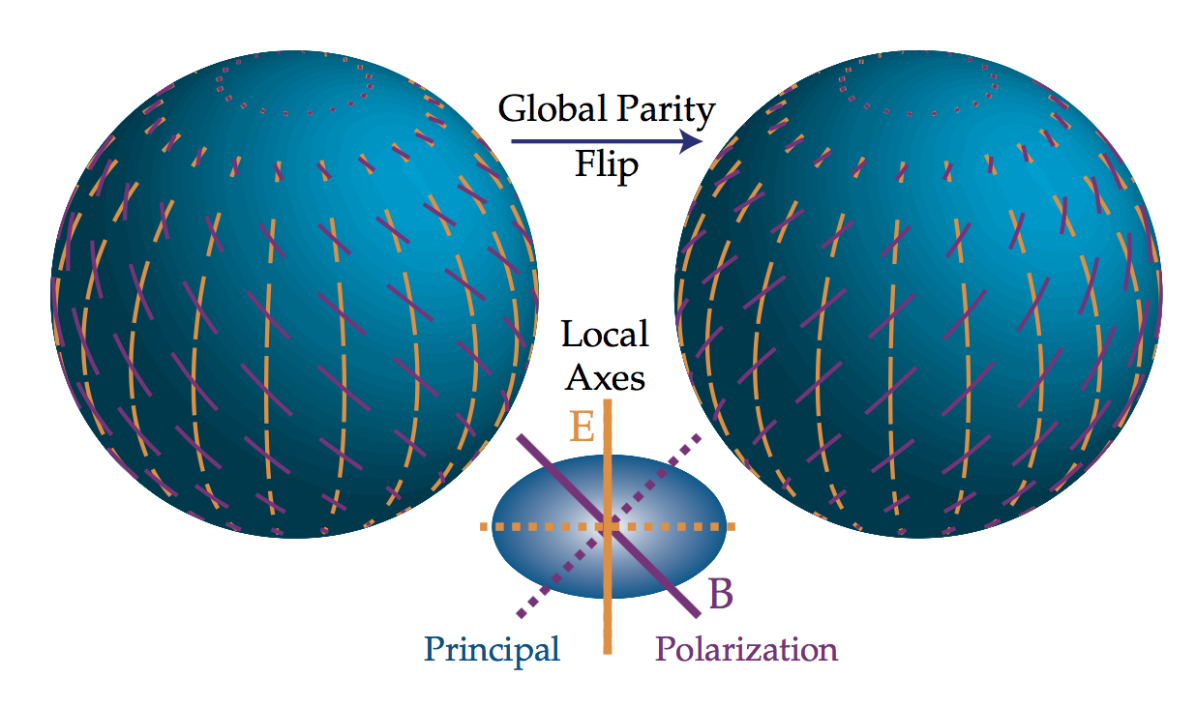
\includegraphics[width=.7\textwidth]{CosmologyPlots/EBmodes.png}
\end{homeworkProblem}
\pagebreak
\begin{homeworkProblem}
   {\color{purple}Our view of the cosmic microwave background is affected by what is along the line of sight. Give two examples of CMB foregrounds that also provide information about the cosmic parameters.}
   \begin{itemize}
       \item It's a long journey from the CMB to us and a lot of opportunity for things to get in the way of CMB photons. Most of it is galactic stuff like like synchotron radiation and dust but some can tell us about cosmological parameters. 
       \item Thermal Sunyaev Zel'dovich $\Rightarrow$ \textbf{ICM scatters photons, shifts BB by optical depth $*$ thermal energy/ rest mass energy. Can measure distance and $\Omega_m$}
       \begin{itemize}
           \item involves scattering of CMB photons by rapidly moving electrons in the hot gas in clusters of galaxies.
           \item It is possible to use a combination of the SZ effect and the X-ray emission from the hot gas to derive a distance to the cluster.\\ This effect is proportional to (1) the number density of electrons, (2) the thickness of the cluster along our line of sight, and (3) the electron temperature. The parameter that combines these factors is called the Kompaneets y parameter, with $y = \tau (kT/mc^2)$. Tau $(\tau)$ is the optical depth or the fraction of photons scattered, while $(kT/mc^2)$ is the electron temperature in units of the rest mass of the electron. 
           \item The SZ effect also amplifies the first peak in the power spectrum which can tell us about $\Omega_m$
           \item The usual order of magnitude for y is about 0.0001, which is very small.
       \end{itemize}
       \begin{center}
            \includegraphics[width=.3\textwidth]{CosmologyPlots/SZ_Effect.PNG}
       \end{center}
       \item Integrated Saches-Wolfe Effect $\Rightarrow$ \textbf{a particle falls into well and expansion makes it easier to get out. Particle gets to keep some energy. Tells us about expansion}
       \begin{itemize}
           \item Light travelling through a supercluster picks up energy in the form of speed and heat like a particle rolling down a valley. 
           \item Normally it would give all that energy back when rolling back up the valley, but dark energy changes the shape of the valley as the particles rolls through it to make it shallower and the particle gets to keep some of that heat. 
           \item It's a gravitational redshift that occurs between the surface of last scattering and the earth but happens when the universe is still dominated by radiation. If the universe were matter dominated than large scale gravitational potential energy wells and hills don't evolve significantly. 
       \end{itemize}
        \begin{center}
        \includegraphics[width=.6\textwidth]{CosmologyPlots/ISW.jpg}
        \end{center}
   \end{itemize}
\end{homeworkProblem}
\pagebreak
\begin{homeworkProblem}
   {\color{purple}Describe cosmological inflation. List at least three important observations it is intended to explain.} \\
   \solution\\
   Inflation occured $10^{-36}$ to $10^{-34}$ seconds after the big bang. Began when quantum fluctuations allowed a small region of space to enter a true vacuum state in a universe otherwise filled with false vacuum. The conceptual part of this is tricky. A simple approach is that the universe was temporarily dominated by a positive cosmological constant $\Lambda_i$ with $w=-1$. \\
   Relevant Equations
   \begin{itemize}
       \item $a(t)=e^{H_it}$ 
       \item $w = p/\rho$, $\rho\propto a^{-3(1+w)}$ with $w=-1$
   \end{itemize}
   Important Observations
   \begin{itemize}
       \item Flatness Problem $\Rightarrow$ The Universe is nearly flat today, and even flatter in the past. Seems fine tuned.
       \begin{itemize}
           \item We can write the friedman equation as $1-\Omega(t)=\frac{H_0^2(1-\Omega_0)}{H(t)^2a(t)^2}$
           \item $\Omega(t)=1$ is unstable equilibrium. Any deviation from this would quickly make things less flat. 
           \item Inflation reduces the dependence of the current flatness on the initial conditions.
       \end{itemize}
       \item Horizon Problem $\Rightarrow$ How is the Universe so homogeneous if not all particles are in causal contact?
       \begin{itemize}
           \item Distance to last scatter $d_p(t_0)=c\int_{t_{ls}}^{t_0}\frac{dt}{a(t)}$, but $t_{ls}<<t_0$ only slightly smaller than current horizon distance.
           \item If you look at two points seperated by 180 degrees on the sky, their current proper distance is $\approx 2d_{hor}(t_0)$, hence they are causally disconnected.
           \item CMB measurements shows that those particles are the same temperature to within one part is $10^5$. How are they in thermal equilibrium?
           \item Universe is matter dominated at last scattering, $a=(3/2H_0t)^{2/3}$, you can get the angular diameter distance $d_a= \frac{c}{1+z} \int \frac{dz}{H(z)}$, which shows you that anything not in a 2 degrees radius is not in causal contact and $d_{hor}(t_{ls})\approx 0.4\text{ Mpc}$.
           \item If you factor in inflation and allow 100 e-foldings $d_{hor}(t_{ls})\approx 10^{43}\text{ Mpc}$ allowing the last scattering surface to be in causal contact.
       \end{itemize}
       \item Monopole Problem $\Rightarrow$ Where are the magnetic monopoles?
       \begin{itemize}
           \item It would be beautiful if all of the forces were originally unified in the beginning of the universe when temperatures were high enough. We know that the electromagnetic and weak forces become the same force as super high temperatures so it's not an insane idea. However one of the predictions of this is that at one point the universe would have been dominated by magnetic monopoles since they occur at every defect in the quantum field and as far as we know, they don't exist. 
           \item Inflation dillutes the number of magnetic monopoles to the point of near non existance. 
       \end{itemize}
   \end{itemize}
\end{homeworkProblem}
\pagebreak
\begin{homeworkProblem}
   Define and describe a `fine tuning problem'. How do anthropic arguments attempt to resolve it?\\
   \\
   \solution \\ 
   \\
   \textbf{Fine Tuning Problem \\ }
   Generally, a fine tuning problem refers to circumstances when the parameters of a model must be adjusted very precisely in order to agree with observations. \\
   Imagine walking into your boss’ office and finding a pencil balanced on its point. You continue to find this pencil balanced every day for the next year until you finally inquire about its origins. Your boss acknowledges that it is quite remarkable to find the pencil this way, but claims that there is no need to explain its origins since he found it this way when he moved into his office. You would probably not find this answer satisfactory, but, on the other hand, if the pencil had simply been lying there, you probably wouldn’t have asked about it in the first place. \\
   In the case of the flatness problem, the pencil standing up on one end is the fact that $\Omega_0=1$.\\
   To prove that if it's flat now, it must have been flatter in the past: \\
   $H^2=\frac{8\pi G}{3}\rho - \frac{\kappa c^2}{a^2}$, plug in $H^2$ from $\Omega=\frac{\rho}{\rho_c}=\frac{8\pi G}{3 H^2}\rho$ $\Rightarrow$ $\frac{1-\Omega}{\Omega}=\frac{-3\kappa c^2}{8\pi G\rho a^2}$ \\ The very early universe was in the radiation dominated era where $\rho\propto a^{-4}$ and $\a\propto t^{1/2}$ \\ 
   $\frac{1-\Omega}{\Omega}\propto \frac{t}{t_0}\frac{1-\Omega_0}{\Omega_0}$\\
   Current measurements from WMAP produce $\Omega_0=1.002$, if we look at the time when the universe was 1 second year old, $\frac{1-\Omega}{\Omega}\sim 10^{-20}$\\ The reason this is surprising is that it isn't a natural state to be in, in fact its an unstable equilibrium point similar to the pencil. \\
   \\
   \textbf{Anthropic Principle} \\ 
   In the example of the flat universe problem, if you consider other universes that aren’t flat, you quickly find that they aren’t universe’s with life in it. \\
   \\
    \textbf{If the universe is open $\Omega_0<1$,}  the density is insufficient to halt the expansion of the universe resulting from the Big Bang. After only a short period of time the universe would be expanding too quickly for gravitationally bound systems to form. \\ 
    \\
    \textbf{If the universe is closed $\Omega_0>1$}, the density of the universe will halt the expansion of the universe and cause it to collapse at some finite time.\\
    \\
    Since the human population clearly exists, then it must be that the universe is flat. \\
    It is unremarkable that the universe has fundamental constants that happen to fall within the narrow range thought to be compatible with life. \\
    Life happens to exist because of the constants and not the other way around.\\ 
    This is only satisfying if a large number of universe's exist.\\
\end{homeworkProblem}
\pagebreak
\begin{homeworkProblem}
   {\color{purple} Define the two-point correlation function. How is it related to the power spectrum? How is the $C_l$ spectrum of the CMB related to low redshift galaxy clustering?}\\
   \\ 
   \solution \\ 
    \\
   \textbf{Define the two-point correlation function.} \\ 
   Describes the likelihood of finding a galaxy at point X given that another galaxy exists with some characteristic separation. \\ 
   Given some distance what is the probability of finding 2 galaxies separated by that distance? \\ 
   Takes into account the fact that galaxies are not randomly distributed in space but are found in groups and clusters. \\
   The correlation function is obtained observationally by averaging over the density products for a large number of pairs of galaxies with given separation r. \\
   $\xi(r)=(r/r_0)^{-\gamma}$, $\gamma\approx 1.7$ \\
   If galaxies are more concentrated $\xi(r) > 0$ and vice versa. \\
   \\
   \textbf{How is it related to the power spectrum?} \\ 
   The correlation is related to the power spectrum via fourier transform: \\
   $P(k)=2\pi \int_0^\infty dx x^2 \frac{sin(kx)}{kx}\xi(x)$ \\ 
   We can measure the correlation seperation between galaxies and determine the functional form of the power spectrum. \\
   \\
   \textbf{How is the $C_l$ spectrum of the CMB related to low redshift galaxy clustering?}\\
   The relevance of low Z galaxy clustering to the $C_l$ spectrum of the CMB is through secondary anisotropies. Low z galaxies can produce changes to the spectrum via the ISW effect, the SZ effect, and gravitational lensing 
\end{homeworkProblem}
\pagebreak
\begin{homeworkProblem}
   {\color{purple}Consider a cosmological model including a positive cosmological constant. Show that, in such a model, the expansion factor eventually expands at an exponential rate. Sketch the time dependence of the expansion factor in the currently favoured cosmological model.}\\
   \solution \\
   \textbf{The scale factor eventually increases at an exponential rate if the cosmological constant is positive.}\\
   The Friedmann equation is written as: 
   \[(\frac{\Dot{a}}{a})^2=\Omega_ra^{-4}+\Omega_m a^{-3}+\Omega_k a^{-2}+\Omega_\Lambda\]
   For large a, only $\Omega_\Lambda$ is left 
   \[(\frac{\Dot{a}}{a})^2=\Omega_\Lambda\]
   \[\frac{1}{a} da =  \sqrt{\Omega_\Lambda} dt\]
   \[ln(a) =  \sqrt{\Omega_\Lambda} t\]
   \[a =  e^{\sqrt{\Omega_\Lambda} t}\]
   \[a\propto e^t\]
   \textbf{Show the time dependence of the expansion factor in the currently favoured cosmological model.}\\
   \includegraphics[width=.7\textwidth]{CosmologyPlots/ScaleFactor.png}
\end{homeworkProblem}
\pagebreak
\begin{homeworkProblem}
   {\color{purple} Define and describe the epoch of reionization. What are the observational constraints on it?} \\ 
   \\
   \solution \\ 
   The reionization of the universe was due almost exclusively to photo-ionization. \\
   Collisional ionization is ruled out since the ICM wasn't hot enough for efficient collisional ionization. \\
   Reionization took place from $z\sim12-6$ \\ 
   \textbf{Lyman Alpha Forest} \\
   The presence of neutral hydrogen absorbs much more of the lyman alpha series. Direct  observational evidence we have of the existence and properties of the general IGM. \\  
    
   \textbf{Gunn-Peterson Trough of Quasars} \\
   Can constrain the end of reionization. The Gunn–Peterson trough is a feature of the spectra of quasars due to the presence of neutral hydrogen in the Intergalactic Medium (IGM). The trough is characterized by suppression of electromagnetic emission from the quasar at wavelengths less than that of the Lyman-alpha line at the redshift of the emitted light. The discovery of the trough in a z = 6.28 quasar, and the absence of the trough in quasars detected at redshifts just below z = 6 presented strong evidence for the hydrogen in the universe having undergone a transition from neutral to ionized around z = 6. \\ 
   \includegraphics[width=.4\textwidth]{CosmologyPlots/GunnPetersonTrough.jpg}
   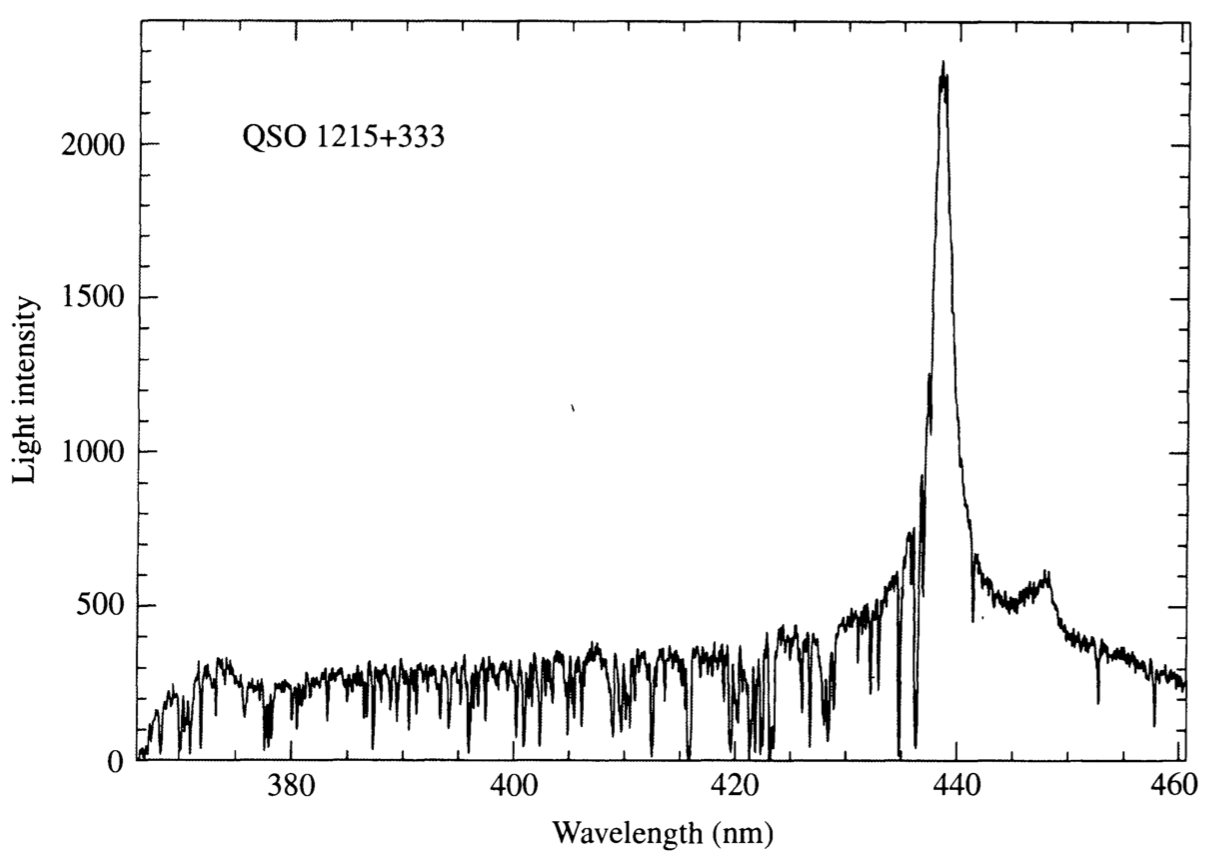
\includegraphics[width=.4\textwidth]{CosmologyPlots/LymanAlphaForest.png}\\
   The top is a close quasar, the bottom is very distant. Note the height of the spectral lines on the left side of  the spectrum. \\
   \textbf{CMB Polarization} \\ 
   Can constrain the beginning of reionization. The degree of polarization from thomson scattering is related to the optical depth and therefore the abundance of free electrons.\\ 
   \textbf{Kinetic SZ Effect} \\ 
   Can tell us how long reionization lasted. The kinetic SZ effect looks at the temperature fluctuations in the CMB. The peculiar velocities of the ionized bubbles produce a doppler shift of CMB photons and the strength of this effect scales with the number of ionized bubbles present. \\
   \textbf{21 cm Spin Flip } \\
   This is the only way to probe the dark ages from recombination to reionization. It can provide a picture of the matter power spectrum after recombination as well as providing the picture for how the universe was reionized. In the late ($z<9$) reionization epoch the 21 cm line is proportional to ionized fraction of hydrogen. 
  
\end{homeworkProblem}
\pagebreak
\begin{homeworkProblem}
   {\color{purple}The 21 cm line of hydrogen is expected to show up in absorption against the cosmic microwave background at some redshifts, and in emission at other redshifts. What physical processes lead to this behaviour?}
\end{homeworkProblem}
\pagebreak
\begin{homeworkProblem}
   What is the difference between scalar and tensor modes of perturbation in the early universe, and how can you detect their presence?
\end{homeworkProblem}
\begin{homeworkProblem}
   What are the similarities and differences between the cosmic neutrino background and he cosmic microwave background?
\end{homeworkProblem}
\begin{homeworkProblem}
   What is the difference between an isocurvature mode and an adiabatic mode, in terms of the initial density perturbations in the early universe? How do we know that the initial conditions are mostly adiabatic?
\end{homeworkProblem}
\begin{homeworkProblem}
   {\color{purple}What is freeze out? Compute the time at which was at a temperature of 1 MeV. Why is this an important time/temperature in cosmology? }\\ 
   \solution \\
   Freeze out is the time where relic abundances of elements cease to change. 
\end{homeworkProblem}
\begin{homeworkProblem}
   Discuss the simple harmonic oscillator picture of the CMB and how the matter density,the baryon density, the radiation density and the curvature affect the CMB power spectrum.
\end{homeworkProblem}
\begin{homeworkProblem}
   What is the integrated Sachs Wolfe effect, and how does it constrain the dark energy density?
\end{homeworkProblem}
\begin{homeworkProblem}
   How is the Boltzmann equation used to compute the relative number densities in the universe? Describe the procedure you would use to set up a set of Boltzmann equations
\end{homeworkProblem}
\begin{homeworkProblem}
   Describe linear perturbation theory and its relevance to studying the evolution of structure in the universe.
\end{homeworkProblem}
\begin{homeworkProblem}
   Write down the general growth equation, and discuss what assumptions we employ to solve for the growth of density perturbations in a matter dominated universe. How do structures grow in a radiation dominated universe?
\end{homeworkProblem}
\begin{homeworkProblem}
   Discuss bias in relation to the constraining the growth of structure.
\end{homeworkProblem}
\begin{homeworkProblem}
   Compare different reionization probes: Lyman alpha absorption from quasars, neutral hydrogen and the CMB polarization
\end{homeworkProblem}
\begin{homeworkProblem}
   Describe Silk damping and what we can learn about cosmological parameters from the CMB tail
\end{homeworkProblem}
\begin{homeworkProblem}
   Discuss three ways of constraining the Hubble constant, and possible degeneraciesbetween the methods.
\end{homeworkProblem}
\begin{homeworkProblem}
   Derive the equation for an Einstein ring for a point mass and discuss how things changewhen the lens is extended.
\end{homeworkProblem}
\begin{homeworkProblem}
   What are some of the systematics in measurements of weak lensing? If they can be controlled, how are they accounted for?
\end{homeworkProblem}
\begin{homeworkProblem}
   {\color{purple}Discuss some of the systematics in supernova measurements. If they can be controlled, how are they accounted for?}
   \begin{itemize}
       \item K-correction: The cosmological redshift affects the measurement of an object’s spectrum because these observations are usually made within a specific wavelength region. For example, observations made with the V-band at 550 nm can be affected as the cosmological redshift brings shorter-wavelength radiation into the V band. This effect can be corrected by adding a compensating term called the K-correction to equation (91) if the spectrum, Iλ, of the object is known.
       \item UV Spread: Type Ia have a higher spread in the UV than in the optical or IR, which becomes problematic when cosmological expansion shifts the U band into the B band.
       \item Reddening: Intrinsic reddening of the SNe themselves and reddening due to dust should be handled separately, but in practice they are hard to deconvolve. Intrinsically fainter SNe Ia are redder than brighter ones, but the same effect occurs with dust extinction.
       \item  Galactic Evolution: It is now well known that fainter SNe Ia tend to be embedded in older stellar populations; this translates to a $\sim 12\%$ brightness increase for $z = 1$ SNe Ia due to increased star formation.

   \end{itemize}
\end{homeworkProblem}
\begin{homeworkProblem}
   How are Fisher matrices used to forecast constraints in cosmology? Describe the difference between Fisher matrix techniques and Markov Chain Monte Carlo methods.
\end{homeworkProblem}
\begin{homeworkProblem}
   What is a degeneracy direction? Given an observable f(x,y), how would you compute the degeneracy direction between parameters x and y?
\end{homeworkProblem}
\pagebreak
\\
\section{Memorize }\\
\\
Mean cmb photon energy $E\sim2.7k_BT$\\
Kelvin Boltzman $k_B=\num{8.6e-5}$eV k$^-1$, this is one thing we could assume is 1\\
Radiation dominated, $a \sim t^{1/2}$\\
Matter dominated, $a\sim t^{2/3}$
\\
\section{Lingering Questions }\\
\\
What is the difference between photodissociation and ionization? \\ 
\section{Assumptions }\\
\subsubsection{Why can we assume that the Universe is homogeneous on large scales?}
The largest gravitationally bound things are galaxy clusters on the order of $R\sim100$ Mpc/h\\
The hubble radius is $R_H=\frac{c}{H_0}=\frac{\num{3e5}km/s}{100 h km/s/Mpc}\sim 3000$ Mpc/h. \\
If we consider the volumn of gravitationally bound things to the rest of the universe: \\
$(\frac{200 Mpc/h}{3000 Mpc/h})^3\sim0.0\bar{6}^3\sim\num{2e-4}$. This assumption is justified.
\section{Sources}
This work is based on or taken from the work of Miranda Herman, Jeffrey Emberson, and Ned Wright
\end{document}
